% ***************************************************************************************
% ************************************* CAPÍTULO I **************************************
% ***************************************************************************************
\chapter{** TITULO DEL CAPÍTULO 1 **}
\thispagestyle{empty}

\abovedisplayskip=0pt
\belowdisplayskip=10pt
\abovedisplayshortskip=0pt
\belowdisplayshortskip=10pt

\epigraph{\flushright El auténtico pensar, como el vivir, es tarea que se aprende. Quien aprende, debe dialogar con
aquellos que han pensado previamente: recorrer sus itinerarios, seguir sus rutas y estelas, consultar
sus bitácoras}{\textit{Ernesto Mayz Vallenilla}\\Rector fundador de la USB}

** COLOQUE AQUÍ CONTENIDO RESPECTIVO **\\

** A CONTINUACIÓN SE HACE UN RESUMEN DE LAS PRINCIPALES HERRAMIENTAS NECESARIAS PARA ESCRIBIR SU LIBRO DE PROYECTO DE GRADO. EL OBJETIVO DE ESTO ES AHORRAR LA MAYOR CANTIDAD DE TIEMPO EN EL \textit{LAYOUT}, ENFOCANDO LOS ESFUERZOS EN EL CONTENIDO DEL PROYECTO **

\section{Figures}

\subsection{Referenciado y posicionamiento de imagenes}

En la figura \ref{fig:cromovegetal} se observa el jardín cromovegetal, concebido por Carlos Cruz-Diez en 1991 en su visita a la Universidad Simón Bolívar.

% for a correct image positioning is important to use the parameters [H], [h] and [p] in a right way.
% The first one place the image in the exact position that is in the LaTeX code
% The second one place the image where the compiler configurate as "best position"
% The last one utilize an entire page for figure positioning

\begin{figure}[H]
\centering
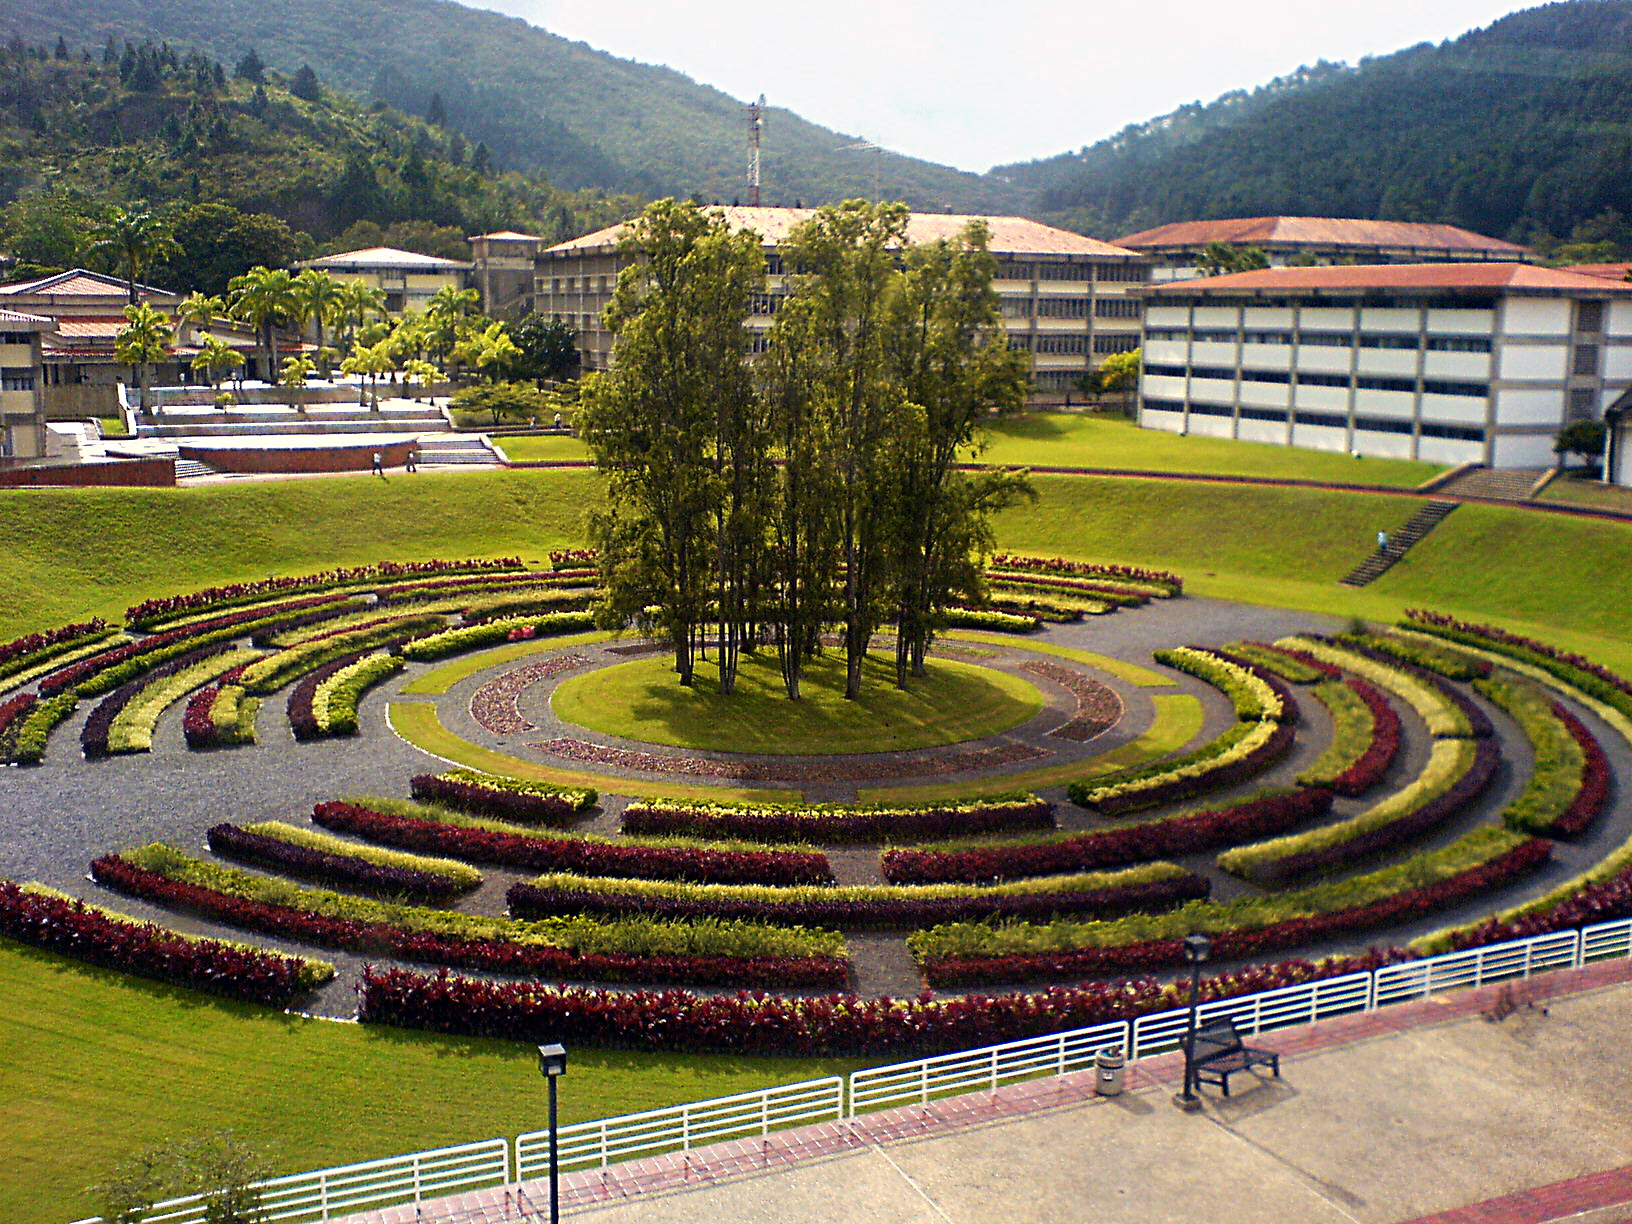
\includegraphics[width=0.50\textwidth]{2_MainMatter/Capitulo1/Imagenes/cromovegetal.jpg}
\caption{Jardín cromovegetal de la Universidad Simón Bolívar}
\label{fig:cromovegetal}
\end{figure}

\subsection{Ejemplo de posicionamiento en hoja completa}

La figura \ref{fig:rectorado} muestra el rectorado de la Universidad Simón Bolívar, sede de los principales entes administrativos de la institución.

\begin{figure}[p]
\centering
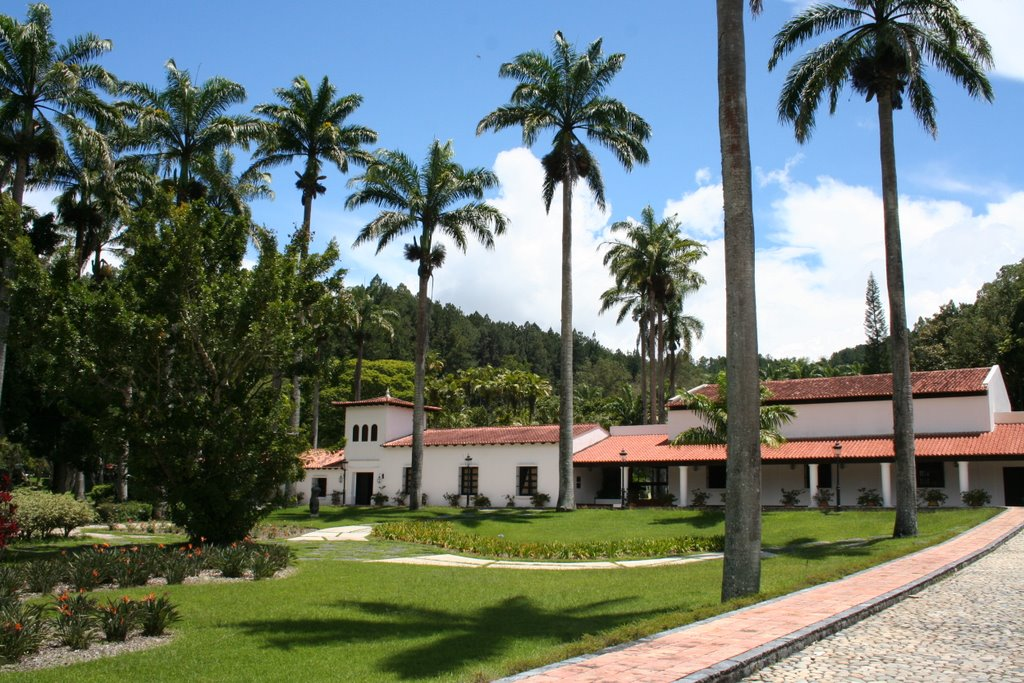
\includegraphics[width=1.0\textwidth]{2_MainMatter/Capitulo1/Imagenes/rectorado.jpg}
\caption{Rectorado de la Universidad Simón Bolívar}
\label{fig:rectorado}
\end{figure}

\subsection{Ángulo de giro en imágenes con orientación horizontal}

La figura \ref{fig:biblioteca} muestra la biblioteca de la USB, lugar de estudio e investigación de un gran número de miembros de la comunidad universitaria.

\begin{figure}[p]
\centering
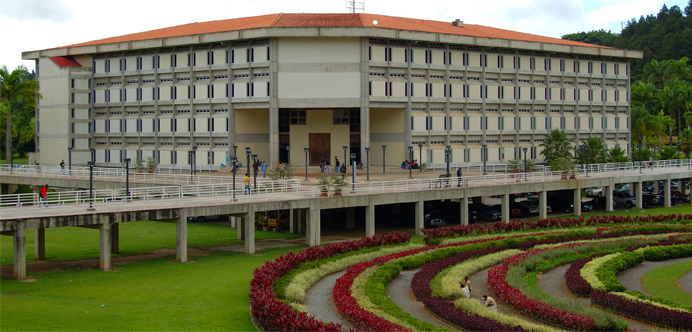
\includegraphics[width=1.3\textwidth, angle=90]{2_MainMatter/Capitulo1/Imagenes/biblioteca.jpg}
\caption{Biblioteca de la Universidad Simón Bolívar}
\label{fig:biblioteca}
\end{figure}

\section{Quotes}

\section{Tables}

\section{Equations}

\section{Programming Code}

\section{Referencias}